\newpage
\section{Algoritmi force-directed de desenare a grafurilor}

Este o categorie de algoritmi de desenare a grafurilor într-un mod plăcut din punct de vedere estetic. 
Printr-un astfel de algoritm se poziționează nodurile grafului într-un spațiu bidimensional sau tridimensional astfel încât 
lungimea muchiilor este mai mult sau mai puțin egală, iar în structura grafului există un număr minim de suprapuneri între muchii, 
iar în cazuri favorabile nici o suprapunere. Desenarea grafurilor poate fi o problema grea de abordat dar prin algoritmii 
de desenare force-directed, se exclud noțiuni ce țin de planaritatea grafurilor, întreaga operație de desenare fiind mai 
degrabă o simulare cu aspecte ce se regăsesc în fizică.\newline

Prin asignarea anumitor forțe setului de noduri și setului de muchii din graf acestea fie se apropie fie se depărtează după 
fiecare iterație a algoritmului, scopul algoritmului fiind de a minimiza deplasarea nodurilor sau a muchiilor până când se 
ajunge la o stare de echilibru. De obicei forțe elastice bazate pe legea lui Hooke sunt atribuite nodurilor unei muchii 
pentru ca acestea să se atragă, în schimb ce simultan forțe de repulsie, similare cu cele ale particulelor cu sarcina electrică 
bazate pe legea lui Coulomb, sunt folosite pentru a crea o repulsie între nodurile grafului. In stările de echilibru ale acestui sistem de forțe, 
muchiile nodurilor care au un părinte comun au de obicei lungimea aproape egala (datorită forței elastice de atracție), 
iar nodurile care nu sunt conectate printr-o muchie se resping între ele (datorită forței de repulsie). Forțele de atracție și repulsie pot fi definite și prin funcții 
care nu sunt bazate pe legile fizice ale elasticității sau sarcinii electrice, de exemplu unele sisteme pot folosi funcții de 
atracție logaritmice în loc de funcții liniare. \newline

\begin{figure}[H]
    \begin{center}
        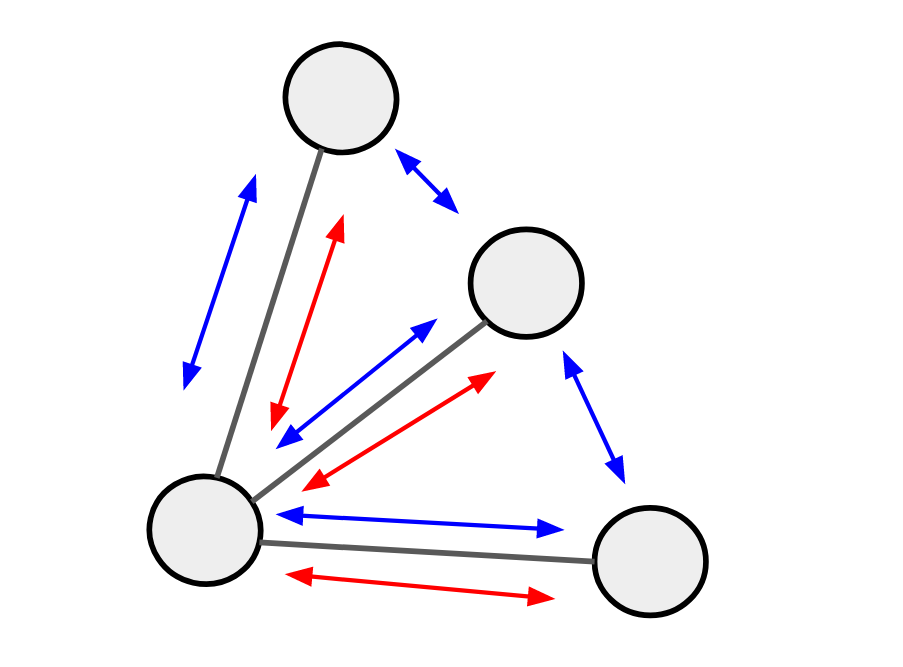
\includegraphics[scale=0.3]{imagini/force/force.png}        
    \end{center}
    \caption{Exemplu pentru aplicarea forțelor. Forța de repulsie între toate nodurile (cu albastru) și forța de atracție între nodurile adiacente (cu roșu).}
    \label{fig:force}
\end{figure}

O forță similară cu cea a gravitații poate fi folosită pentru a atrage nodurile către un punct fix în planul de desenare, 
astfel pentru un graf cu mai multe componente conexe acestea vor sta relativ în aceeași zonă și nu se vor mai depărta 
constant una de cealaltă datorită forței continue de repulsie și a lipsei de atracție între ele. Forțe similare cu cele 
magnetice pot fi aplicate într-un sistem, atât pe noduri cât și pe muchii în sine, pentru a evita suprapunerea muchiilor 
în întreaga simulare. \cite{force2}\newline

\subsection{Aplicare}

Odată ce forțele au fost atribuite nodurilor sau muchiilor dintr-un graf, întregul comportament al elementelor 
este simulat ca într-un sistem fizic unde nodurile se deplasează la fiecare iterație. Acest proces este repetat 
iterativ până când se ajunge la o stare de echilibru mecanic, adică pozițiile relative ale elementelor nu se mai 
schimbă de la o iterație la alta. Structura finală după întregul proces este folosită pentru a reprezenta graful ce 
trebuie desenat.\newline

Este posibilă și adăugarea unui mecanism de calculare a stării de echilibru pe lângă simularea fizică, acestea fiind 
metode de optimizare globală, precum algoritmi genetici.\newline

\subsection{Avantaje}
\begin{itemize}
\item Rezultate calitative

Pentru grafuri de mărimi medii (50-500) de noduri de multe ori rezultatul aplicării unui algoritm force-directed este 
unul bun și inteligibil din perspectiva omului. Rezultatul fiind catalogat după următoarele criterii: 
\begin{itemize}
    \item lungimea uniformă a muchiilor
    \item distribuirea uniformă a nodurilor
    \item număr minim de suprapuneri
    \item simetrie
\end{itemize}

Simetria este un criteriu greu de îndeplinit și depinde de structura internă a grafului.
\item Flexibilitate

Algoritmul ales poate fi adaptat pentru a îndeplinii criterii adiționale de desenare. 
Exemple de extensibilitate ar fi desenarea de: grafuri orientate, grafuri 3D, grafuri împărțite în clustere, multigrafuri, grafuri ponderate

\item Intuitivitate

Având la bază analogii din fizică, precum elasticitatea, comportamentul algoritmului este ușor de prezis și înțeles.
\item Simplitate

De obicei astfel de algoritmi sunt ușor de implementat, sau au fost deja implementați în anumite biblioteci.
\item Interactivitate

Prin desenarea unor stagii intermediare ale grafului pe care este aplicat algoritmul, utilizatorul poate urmării evoluția 
procesului, observând cum se dezvoltă dintr-o structura încurcata cu multe suprapuneri de muchii, într-un graf echilibrat 
și ușor de urmărit.
\item Fundație teoretică

Înca din anii 1960 metode de desenare ale grafurilor au fost cercetate, o primă implementare fiind făcuta 
prin algoritmul lui Tutte în anul 1963 folosind o reprezentare baricentrică (prin care se seteaza un grup de noduri 
de baza în jurul cărora celelalte noduri vor fi plasate), folosind doar forte de atracție. 
În următorii ani alte metode de desenare au fost create de către Eades(1984), Fruchterman și Reingold (1991), Kamada și Kawai (1989).

\end{itemize}

\subsection{Dezavantaje}

\begin{itemize}
\item Timp de rulare mare

De obicei complexitatea unui algoritm de desenare force-directed este \(O(n^3)\), unde \(n\) este numărul de noduri din graf. 
Acest lucru rezultă deoarece numărul iterațiilor este estimat ca fiind \(O(n)\) iar pentru fiecare iterație fiecare 
pereche de noduri trebuie vizitată pentru calcularea forței de repulsie mutuale.

\item Minim local

Prin algoritmii force-directed se ajunge la o structură în care nodurile se află într-o stare de echilibru, întreg procesul poate 
fi considerat ca fiind rezolvarea unei probleme de optimizare.
De cele mai multe ori starea rezultată se poate afla într-un minim local al funcție ce trebuie optimizate, dar care nu 
coincide neapărat cu un minim global. Întreg procesul depinde de starea inițială a nodurilor care este aleasa aleatoriu. 
Această problemă crește odată cu numărul de noduri din graf. O modalitate de rezolvare ar fi combinarea a mai multor 
algoritmi force-directed pentru obținerea unui rezultat mai bun. De exemplu folosirea algoritmului Kamada–Kawai pentru 
crearea unei așezări în plan inițiale, iar apoi îmbunătățirea structurii cu ajutorul algoritmului Fruchterman–Reingold.

\end{itemize}

\subsection{Metode de desenare}
\subsubsection{Metoda baricentrică}
Metoda baricentrică de desenare a lui Tutte din 1963 este considerată prima versiune a unui algoritm force-directed 
pentru obținerea unei structuri cu muchii drepte, fără suprapuneri pentru un graf planar 3-conex. În comparație cu alte 
metode de desenare această varianta garantează că fețele grafului planar sunt convexe. Idea în spatele algoritmului 
constă în faptul că dacă o față a grafului planar este fixată în plan, atunci pozițiile potrivite ale celorlalte noduri sunt 
găsite rezolvănd un set de ecuații liniare, unde fiecare poziție a unui nod este reprezentata ca o combinație convexa a 
pozițiilor nodurilor vecine lui. In acest model forța unei muchii \((u,v)\) este direct proporțională cu distanța dintre 
nodul \(u\) și \(v\) in plan. Astfel forța la un nod \(v\) este descrisa prin 
\[F(v)=\sum_{(u,v) \in E} p_u-p_v\] 
unde \(p_u\) și \(p_v\) sunt pozițiile nodurilor. Deoarece această funcție are un minim cu toate nodurile așezate în aceeași locație, setul 
de noduri trebuie împărțit în noduri fixe și noduri libere, care pot fi deplasate. \cite{force}

\begin{algorithm}[H]
    \caption{Metoda baricentrică de desenare \cite{force}}
    Input: \(G=(V,E)\);\newline
    partiționarea lui \(V\) într-un set \(V_0\) cu cel puțin 3 noduri fixe și un set \(V_1\) cu noduri libere, \(V=V_0 \cup V_1\);\newline
    un poligon convex \(P\) cu \(|V_0|\) vârfuri.\newline

    Output: o poziție \(p_v\) pentru fiecare nod din \(V\) astfel încat nodurile fixe formeaza un poligon.
        
    \begin{algorithmic}[1]
        \State Plasează fiecare nod \(u \in V_0\) la un varf al lui \(P\), și fiecare nod liber în origine
        \Repeat
        \ForEach{ \(v \in V_1 \) }
            \State \(x_v=\frac{1}{deg(v)} \sum_{(u,v) \in E} x_u\)
            \State \(y_v=\frac{1}{deg(v)} \sum_{(u,v) \in E} y_u\)
        \EndFor
        \Until{ \(x_v\) și \(y_v\) converg pentru toate nodurile libere \(v\)}
    \end{algorithmic}
\end{algorithm}

\subsubsection{Algoritmul Fruchterman–Reingold}

Algoritmul Fruchterman-Reingold de desenare a grafurilor introduce noțiunea de temperatură. Această variabilă are o valoare setată 
la început iar ea scade la fiecare iterație pana la \(0\). Temperatura controlează deplasarea nodurilor iar cu 
cât ne apropiem de un minim, cu atât temperatura v-a fi mai mică pentru a nu schimba cu mult rezultatul.\cite{force}

\begin{algorithm}[H]
    \caption{Fruchterman si Reingold \cite{force}}
    \(arie=W*L\); \(W\) și \(L\) sunt lățimea și lungimea suprafeței de desenare\newline
    \(G=(V,E)\); nodurile au poziții inițiale aleatorii\newline
    \(k=\sqrt{arie/|V|}\) \newline
    \(f_a(x)=x^2/k\)\newline
    \(f_r(x)=k^2/x\)\newline 
    \begin{algorithmic}[1]
        \For{\(i=1\) to \(iteratii\)}
            \State calcularea forțelor de repulsie
            \ForEach{\(v \in V\)}
                \State fiecare nod are doi vectori \(pos\) și \(disp\)
                \State \(v.disp=0\)
                \ForEach{\(u \in V\)}
                    \If{ \(u \neq v\)}
                        \State \(\delta\) este vectorul diferență dintre pozițiile celor două noduri
                        \State \(\delta=v.pos-u.pos\)
                        \State \(v.disp=v.disp+(\delta/|\delta|)*f_r(|\delta|)\)
                    \EndIf
                \EndFor
            \EndFor

            \State calcularea forțelor de atracție
            \ForEach{\(e \in E\)}
                \State fiecare muchie este o perche de noduri \(u\) și \(v\)
                \State \(\delta=e.v.pos-e.u.pos\)
                \State \(e.v.disp=e.v.disp-(\delta/|\delta|)*f_a(|\delta|)\)
                \State \(e.u.disp=e.u.disp+(\delta/|\delta|)*f_a(|\delta|)\)
            \EndFor

            \State deplasarea maximă se limitează în funcție de temperatura \(t\)
            \ForEach{\(v \in V\)}
                \State \(v.pos=v.pos+(v.disp/|v.disp|)*min(v.disp,t)\)
                \State \(v.pos.x=min(W/2,max(-W/2,v.pos.x))\)
                \State \(v.pos.y=min(L/2,max(-L/2,v.pos.y))\)
            \EndFor

            \State reducerea temperaturii 
            \State \(t=cool(t)\)
        \EndFor
    \end{algorithmic}
\end{algorithm}

  

